% !TEX root = ../thesis.tex

\chapter{Streaming WPS}
\label{sec:streamingwps}

In contrast to conventional data processing, such as the method used in the \ac{WPS}, streaming processing approaches show considerable benefits. Regarding to time efficiency and with reference to the already mentioned problems of processing substantial large data sets or live data, the development of a streaming enabled \ac{WPS} seems to be of great value.

Data streams can be seen as an abstract concept that stands in contrast to conventional batch data. Data streams are (possibly infinite) sequences of data items (or chunks) that become available over time, whereas conventional batch data describes a pile of data that is either completely available or not. The abstract concept of streaming can be observed across different technologies and fields of application. Starting from the concept of pipes and filters on unix-like operating systems, over interprocess communication using sockets \citep[either local or over a network,][]{buschmann1996pattern}, the ubiquitous usage in programming languages (as a concept of I/O or in functional programming languages in the form of inductive data type definitions), \ac{GPGPU} to modern media streaming solutions like RTP, RTCP, RTSP \citep{ietf:rfc3550,ietf:rfc2326} or SIP \citep{ietf:rfc3261}. The best way to illustrate this concept is to look on its most popular usage form: media streaming. The conventional approach to view a video or play a sound file over a network is to download the file and to play it locally. Depending on the encoding and compression which has been applied to the media file, it is not possible to play the file until the download is finished. By sending smaller parts of the media file (e.g. one or more single frames) over the network, the time to start playing is reduced to a great degree. Suitable players are now able to play this stream of frames long before the whole file is transmitted. Besides the on-demand streaming of media (the streamed file is completely available on the remote side), the transmission of live audio or video becomes possible by transferring audio or video frames as soon as they are recorded.

The concept of streaming processing extends this simple pattern by not only accepting a stream of input data, but also by generating a stream of output data. The processing takes place on small chunks of the input data instead of the complete data set. By sequentially processing the stream, software is able to process very large or infinite data sets because the complete data set neither needs to be kept in memory nor it is needed to be stored. This permits the analysis of live data, e.g. the evaluation of continuously collected sensor data. Also the initial response time (the time until the first outputs of a program are available) is equally reduced as in media streaming. Reducing the latency of initial data output has various advantages, e.g. earlier appearance of errors (and by this the possibility to stop processing to save computing resources and time and thus also reducing financial costs) or the ability to develop more responsive end user solutions, e.g. by gradually updating a data visualization instead of presenting the data after waiting for the complete result.

In the case of spatiotemporal data, streaming processing is especially useful and advisable, as data sets tend to become rather large and the analysis of real-time data can have great benefits. Especially as spatiotemporal data is often adequate for streaming: spatial data sets are often aggregates or collections that can be easily broken down into smaller parts (like single features, observations or tiles). On the other side, spatiotemporal data has the salient characteristic of showing strong dependencies to nearby data and thus can be difficult to analyze using non-random-access paradigms like streaming. The case of inter-feature dependencies needs to be considered when transferring the concept of streaming to spatiotemporal processing. Algorithms used in streaming are required to operate on smaller chunks of the complete data set. Computations that require global knowledge are not expected to have any advantage from streaming. For example, graph algorithms like Dijkstra's algorithm \citep{dijkstra} can not start the computation before the complete graph is available.

Streaming processing can be divided into three categories that differ from conventional processing (see \pseudosubfigure{fig:streaming}{a}). Characteristic for input streaming (\pseudosubfigure{fig:streaming}{b}) is the parallel occurrence of input and processing with a subsequent output after processing finished. On the other hand, output streaming processing describes the isolated input supply and parallel processing and output (\pseudosubfigure{fig:streaming}{c}). These two approaches are combined in the third category, full input and output streaming (\pseudosubfigure{fig:streaming}{d}), in which input, processing and output take place concurrently. Despite their respective level of concurrency, all three categories have the very same advantage. By parallelizing processing and input and/or output, the overall execution and initial response time is appreciably shorter. Full input and output streaming enabled processes have the additional advantage to be able to process indefinite large data sets by processing each input data chunk separately and outputting an output data chunk for each of them. Through this, the analysis of live sensor data can be accomplished. Each of these categories of processing demand different requirements from the process or algorithm. To create a stream, the data set needs to be divided into smaller chunks; input streaming enabled algorithms need to be able to operate on each of these chunks separately and output streaming enabled processes need to be able to produce intermediate results. Input streaming would not result in any benefits for algorithms requiring global knowledge of the data set because they can not start processing until all data chunks have been arrived. Processes that result in a single output value, for which the processing has to be completed, offer no advantage when they are output streaming enabled.

\begin{figure}[!htb]
  \centering
  % !TEX root = ../thesis.tex
\begin{tikzpicture}
	\scriptsize
	\tikzset{
	  ibox/.style = {draw, fill=string!50,  minimum width=4cm, minimum height=.6cm},
	  pbox/.style = {draw, fill=comment!50, minimum width=4cm, minimum height=.6cm},
	  obox/.style = {draw, fill=keyword!50, minimum width=4cm, minimum height=.6cm},
	  every node/.style={font=\sffamily},
	}
	\draw[>->] (-2.4,3.6) -- (11.4,3.6);
	%\draw[]   (-2.4,3.6) -- (-2.4, -6);
	\draw[>->] (-2.4, -6) -- (11.4, -6);

	\draw[dotted] (-2.0,-6) -- (-2.0,3.6);
	\draw[dotted] (-1.0,-6) -- (-1.0,3.6);
	\draw[dotted] (-0.0,-6) -- (-0.0,3.6);
	\draw[dotted] (1.0,-6) -- (1.0,3.6);
	\draw[dotted] (2.0,-6) -- (2.0,3.6);
	\draw[dotted] (3.0,-6) -- (3.0,3.6);
	\draw[dotted] (4.0,-6) -- (4.0,3.6);
	\draw[dotted] (5.0,-6) -- (5.0,3.6);
	\draw[dotted] (6.0,-6) -- (6.0,3.6);
	\draw[dotted] (7.0,-6) -- (7.0,3.6);
	\draw[dotted] (8.0,-6) -- (8.0,3.6);
	\draw[dotted] (9.0,-6) -- (9.0,3.6);
	\draw[dotted] (10.0,-6) -- (10.0,3.6);
	\draw[dotted] (11.0,3.6) -- (11.0,-6) node [below] {Time};

	\node [xshift=-1.5cm,yshift=2.4cm] {(a)};
	\node [ibox,yshift=3.0cm,xshift=1cm] (input1) {Input Upload};
	\node [pbox,yshift=2.4cm,xshift=5cm] (processing1) {Processing};
	\node [obox,yshift=1.8cm,xshift=9cm] (output1) {Output Download};

	\draw[dashed] (-2.4, 1.2) -- (11.4, 1.2);

	\node [xshift=-1.5cm,yshift=0cm] {(b)};
	\node [ibox,yshift= .6cm,xshift=1cm] (input2) {Input Stream};
	\node [pbox,yshift= .0cm,xshift=2cm] (processing2) {Processing};
	\node [obox,yshift=-.6cm,xshift=6cm] (output2) {Output Stream};

	\draw[dashed] (-2.4, -1.2) -- (11.4, -1.2);

	\node [xshift=-1.5cm,yshift=-2.4cm] {(c)};
	\node [ibox,yshift=-1.8cm,xshift=1cm] (input3) {Input Stream};
	\node [pbox,yshift=-2.4cm,xshift=5cm] (processing3) {Processing};
	\node [obox,yshift=-3.0cm,xshift=6cm] (output3) {Output Stream};

	\draw[dashed] (-2.4, -3.6) -- (11.4, -3.6);

	\node [xshift=-1.5cm,yshift=-4.8cm] {(d)};
	\node [ibox,yshift=-4.2cm,xshift=1cm] (input4) {Input Stream};
	\node [pbox,yshift=-4.8cm,xshift=2cm] (processing4) {Processing};
	\node [obox,yshift=-5.4cm,xshift=3cm] (output4) {Output Stream};
\end{tikzpicture}
  \caption{\label{fig:streaming}Four different types of processing data: (a) conventional processing, (b) streaming input data (c) streaming output data, (d) full input and output streaming \citep[based on][]{foerster2012live}.}
\end{figure}

While there are efforts to utilize popular techniques like grid and cloud computing, there are few efforts in research and development to facilitate streaming processing \citep{foerster2012live}. Previous approaches to combine the concept of streaming and web-based processing of spatiotemporal data using the \ac{WPS} are drafted in strong correlation to media streaming \citep{foerster2012live} by using playlist files \citep{ietf:draft-pantos-http-live-streaming-12} as inputs and outputs of a \ac{WPS} process. The process is executed asynchronously and the output playlist location is published using the \texttag{wps}{ProcessStarted} element of the process status response (see \cref{fig:sd:previous}). As the \ac{WPS} specification is not designed to be extensible, the element's content is restricted to a simple string and can not contain complex \ac{XML} structures. Furthermore, the element's definition states that it should be used to convey a human readable text that is presented to an user:
\begin{xquote}[\citet{ogc:wps}]
  ``A human-readable text string whose contents are left open to definition by each WPS server, but is expected to include any messages the server may wish to let the clients know. Such information could include how much longer the process may take to execute, or any warning conditions that may have been encountered to date. The client may display this text to a human user.''
\end{xquote}
Despite the goal of maintaining compatibility to \ac{WPS} specification and existing software components, this represents a misappropriation of the element and will result in incompatibilities with existing \ac{WPS} client solutions. Besides that, this solution is only able to transport a single playlist location to the client and thus, a \ac{WPS} process may only have a single streaming output.

\begin{figure}[!htb]
  \centering
  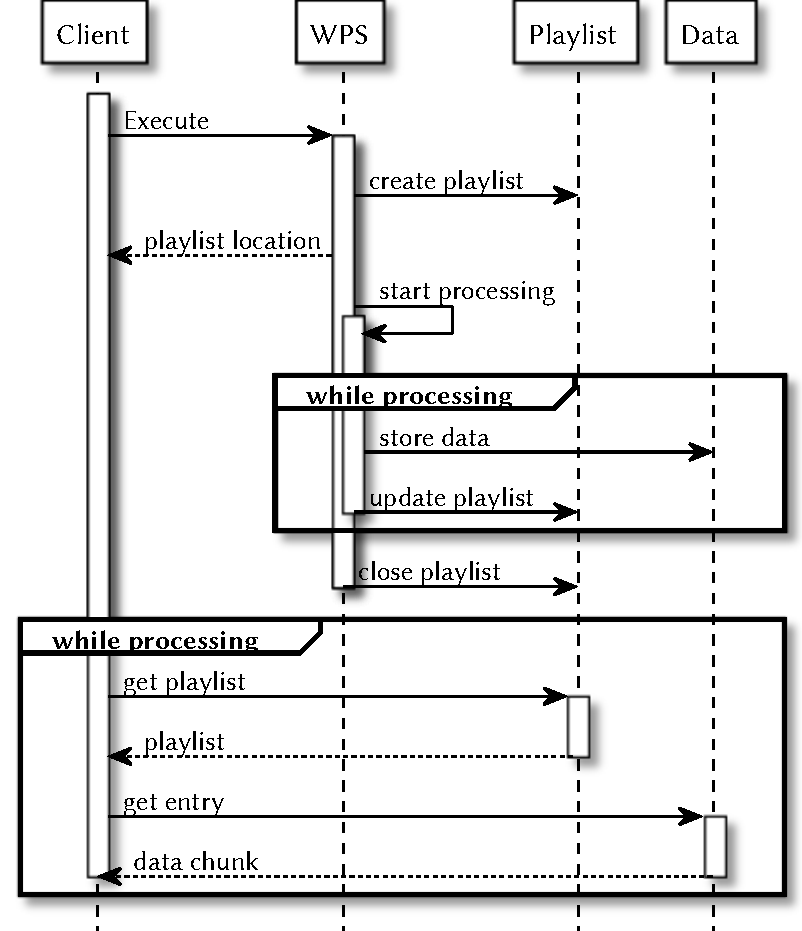
\includegraphics[width = 0.54225352112676062\linewidth]{figures/sequence-diagram-previous.pdf}
  \caption{\label{fig:sd:previous}Sequence diagram of the playlist-based streaming enabled WPS \citep{foerster2012live}.}
\end{figure}

Input parameters may also be supplied using a playlist file. The coordination of several streaming inputs is either not possible or heavily depending on the streaming enabled process. A process accepting two ore more streamed data sets has to decide which data chunks it has to combine. Even the simplest case of combining chunks with the same index of both streams can have serious implications in the use case of live analysis. If a data chunk gets lost, either due to hardware or network failure, the process will combine chunks that are not related. In continuous processes this error can not be detected because two indefinite streams of data will always have matching indices. Use cases, in which the rate of incoming data differs between streams or in which data chunks depend on other chunks, are very hard to model and will result in highly specialized processes. These models depend not only on the structure and format of input data, but also on the data source, and thus the incoming rate of the data. By this, generic solutions, that convert existing \ac{WPS} processes into streaming enabled processes, are hard to develop, and most streaming enabled processes may not be used in contexts apart from the one that it was developed for.

Moreover, realizing streaming by continuous polling of playlists is highly inefficient. Neither can the client know the rate output data is produced nor can the \ac{WPS} process know at which rate input data becomes available. By polling at a too slow rate the arrival of data chunks may be missed, which results in a slower process execution, and by polling at a too high rate, network and computation resources are wasted. Adaptive polling rates may be a solution for this problem, but are useless in cases, where the rate of incoming data changes across the process execution. In contrast to transporting data from the server to the client, for which the playlist concept was originally developed in the context of media streaming, the usage of playlists to transport data from the client to the server is additionally questionable. Clients need the capability to publish files as resources, which are accessible using an URL (e.g. on a FTP or HTTP server). In a web browser environment, a JavaScript client is only able to do this using an external service that stores the data and maintains the playlist. A pure JavaScript browser client is not able to use streaming inputs in this playlist-based streaming \ac{WPS} approach. The implementation of this approach is additionally limited. Input parameter data streams are not implemented and process implementations have to split inputs to create output streams (see \cref{fig:streaming}c). Splitting spatiotemporal data into smaller chunks is not as trivial as e.g. splitting an audio or video stream into single frames. By this, the process implementations become heavily format dependent and dependencies between data chunks can only be expressed as part of the data, and in a format, that the process is able to understand and to handle. Also this approach requires a reimplementation of already existing processes to achieve streaming outputs.

A streaming enabled \ac{WPS} should extend the traditional processing paradigm (see \pseudosubfigure{fig:streaming}{a}) to enable input only streaming (\pseudosubfigure{fig:streaming}{b}), output only streaming (\pseudosubfigure{fig:streaming}{c}), and full input/output streaming (\pseudosubfigure{fig:streaming}{d}). For this, it should be possible to supply input parameters subsequently and to publish output data chunks as they become available. To accomplish this, a streaming enabled \ac{WPS} should not rely on inefficient polling techniques, in which the server or client is requesting a resource continuously over time, but should rely on true streaming technologies that offer a full-duplex communication channel between client and server. Streaming enabled processes should be accessible from the same environments as conventional \ac{WPS} processes. This especially includes web browser environments that are particularly restricted in their possibilities. A streaming enabled \ac{WPS} process should rely on existing, widely known and standardized technologies, it should be especially as interoperable as possible to the \ac{WPS} specification, but should not compromise streaming functionality by enforcing incompatible standards. As spatiotemporal data and its processing and analysis often can not be treated independently from surrounding data, dependencies between streamed data chunks have to be considered. This will require the streaming enabled process to be able not only to operate on sequential data but also be able to allow, to some degree, random access to the data. Despite handling of dependencies between spatiotemporal features should be considered, processes and algorithms that require global knowledge of the data set, may not profit from streaming and should not be considered relevant for a streaming enabled \ac{WPS}. The system should be as generic as the existing \ac{WPS} specification, so it should not rely on specific data formats and allow easy chaining of streaming processes. As possible use cases include not only live analysis of data, but also the processing of large data set, data chunks should be processed in parallel if possible. As this may result in an undefined order of outputted data chunks, clients need to be able to correlate output data chunks with the input parameter chunks. Existing \ac{WPS} processes should be easily converted to streaming enabled processes, without the need to develop them from scratch.

The following sections should introduce a approach for a Streaming \ac{WPS}, that will fulfill the above requirements. As seen in previous approaches, the constraints imposed by the \ac{WPS} specification are too strict to implement a standard compatible streaming enabled WPS fulfilling the requirements. Previous solutions compromised functionality for the sake of (incomplete) compatibility with the inflexible standard. In order to enable true, browser compatible streaming, the approach presented in thesis will break out of the constraining \ac{WPS} standard and develop a message-based architecture using WebSockets to accomplish true full-duplex streaming of data while reusing terminology and technology specified by the \ac{WPS} standard.

\section{Protocol}
  As the \ac{WPS} specification is not flexible enough to model a full streaming scenario, the \ac{WPS} needs to be bypassed. In order to accomplish this, a more flexible interaction model was developed, which extends the conventional processing approach. This protocol is message-based and enables full-duplex stream processing of spatiotemporal data. A \emph{streaming enabled algorithm} is a \ac{WPS} algorithm that supports the here defined protocol while a \emph{streaming process} is the identifiable instance of an algorithm, created by executing the streaming enabled algorithm using the \ac{WPS} \emph{Execute} operation. The streaming process is the core of the Streaming \ac{WPS} and receives subsequent inputs and will emit intermediate results. The execution of the streaming enabled algorithm is fully supported by the \ac{WPS} specification, whereas all interaction with the streaming process is not part of the standard. To communicate with the streaming process, the client needs information on how to connect to the process. As the \ac{WPS} specification does not allow subsequent outputs, the call of the \emph{Execute} operation will return immediately to transport this information to the client, and can not persist over the lifetime of the streaming process.

  To enable a full duplex communication with the streaming process, WebSockets will be used to transport messages. They are needed to \emph{push} messages to clients instead of letting the clients constantly request updates.

  \begin{figure}[!htb]
    \centering
    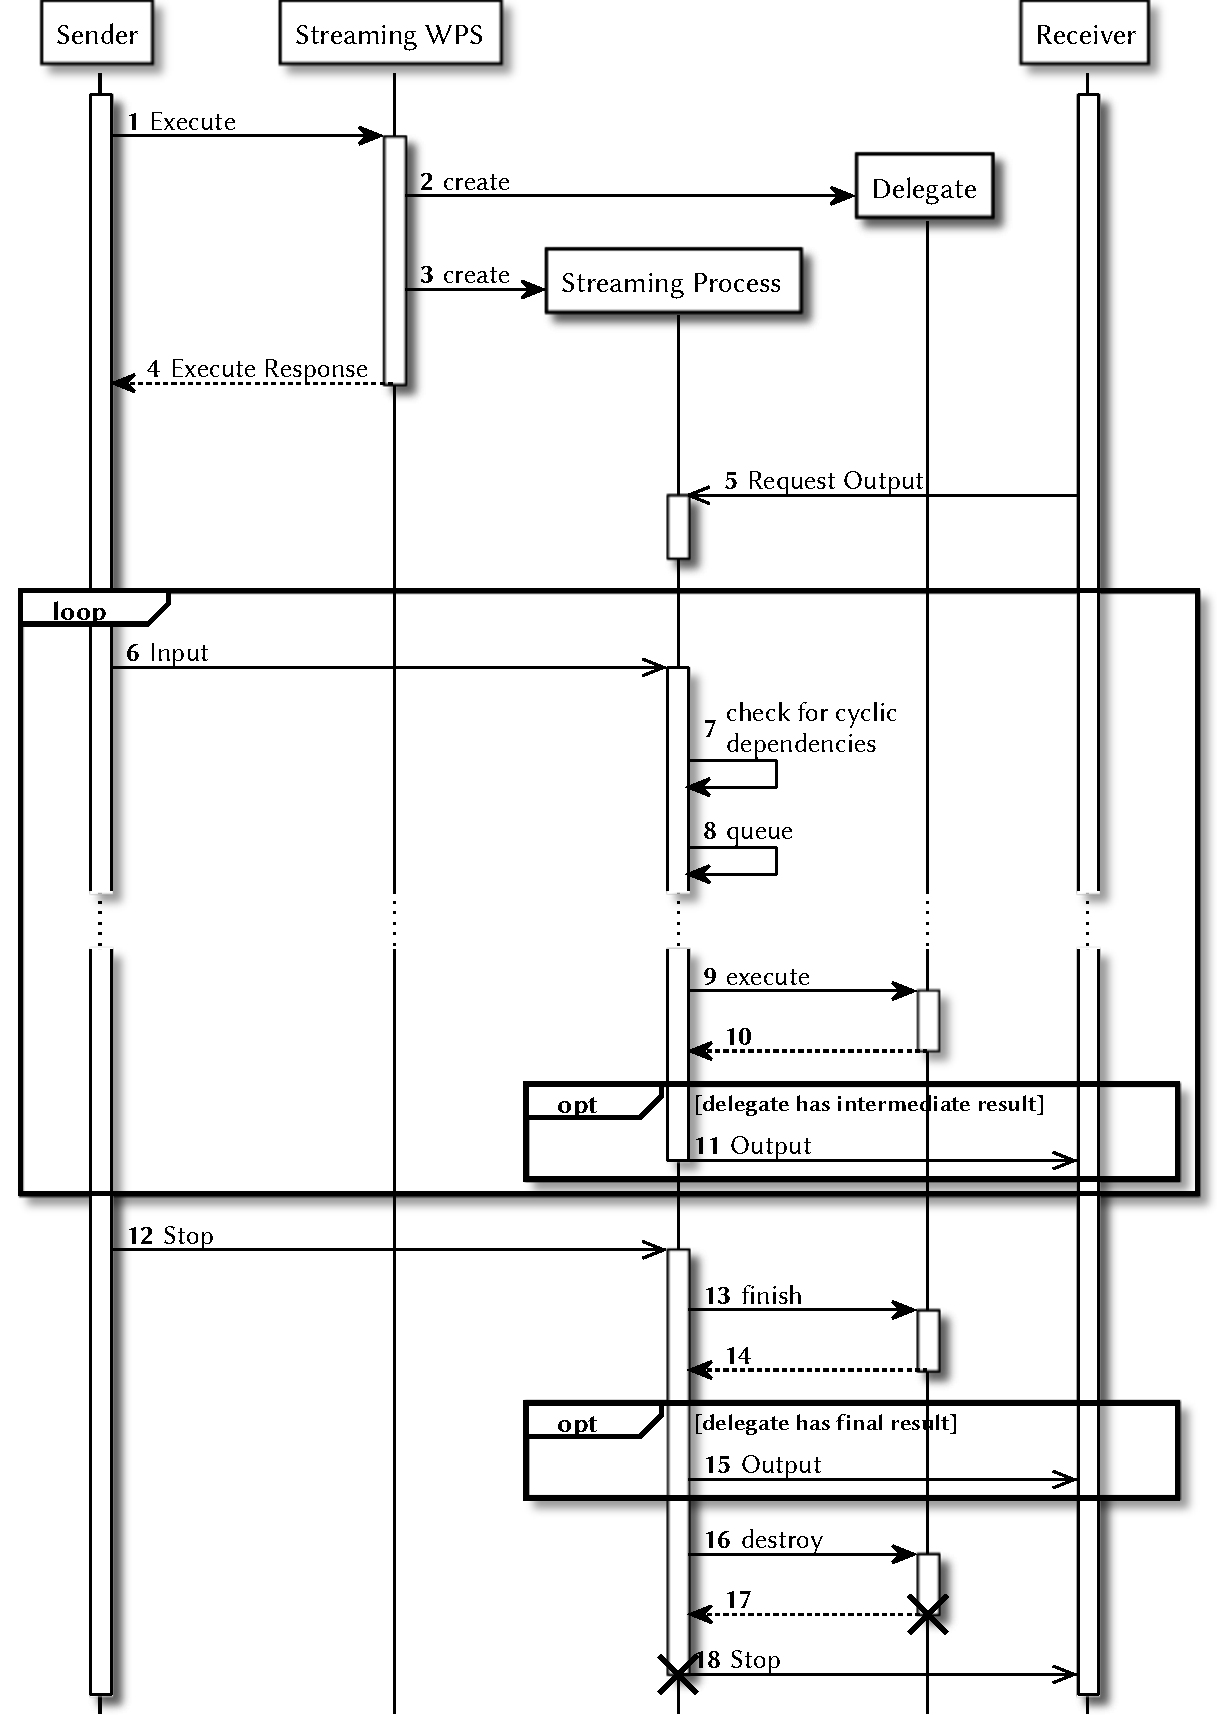
\includegraphics[width = 0.82253521126760565\linewidth]{figures/sequence-diagram-swps.pdf}
    \caption{\label{fig:sd:swps}Sequence diagram of typical interaction pattern with a streaming enabled WPS algorithm using two distinct clients for sending and receiving data.}
  \end{figure}

  The detailed interaction protocol is depicted in \cref{fig:sd:swps}. A client (\emph{Sender}) issues an \emph{Execute} to a streaming enabled WPS algorithm (\step{fig:sd:swps}{1}). The algorithm instantiates a delegate (\hyperref[fig:sd:swps]{step 2}) that is responsible for processing data chunks, and a streaming process (\hyperref[fig:sd:swps]{step 3}) that is responsible for client interactions and task scheduling. The Execute response will contain the necessary details to connect to the streaming processes, such as the the identifier of the streaming process and the WebSocket endpoint URL (\step{fig:sd:swps}{4}).

  With these details a client can connect directly to the streaming process bypassing the \ac{WPS} interface. In \step{fig:sd:swps}{5} another client\footnote{Even though sender and receiver are two different entities in this diagram, there are no restrictions imposed to the amount of clients, either senders or receivers, or their nature (senders may also be receivers).} (\emph{Receiver}) connects to the streaming process and subscribes to the future outputs of the process. By this, the client does not need to constantly issue requests to the streaming process to check for new outputs, but receives outputs automatically as long as the receiving client stays connected using the WebSocket. After this, one or multiple clients start sending chunks of data as input parameters to the streaming process (\step{fig:sd:swps}{6}). The clients may open a new connection for every input or use the same connection over the lifetime of the streaming process. The streaming process checks the inputs for validity (\step{fig:sd:swps}{7}) and queues them for processing (\step{fig:sd:swps}{8}). Processing takes places asynchronously in parallel manner and there is no guarantee of order (besides restrictions imposed by dependencies, see \cref{sec:stream:input:reference,sec:stream:dependencies}). When there are free capacities to process the data and all other requirements are met, the delegate is tasked to process the data (\step{fig:sd:swps}{9}). The delegate implementation can return an intermediate result in \step{fig:sd:swps}{10}, which is forwarded to all registered receivers in \step{fig:sd:swps}{11}. \Steprange{fig:sd:swps}{6}{11} may be repeated indefinitely (e.g. live analysis of data) or until the sending client has no more inputs to feed. As the streaming process would wait in this case forever (or at least until some timeout interferes), the client has to stop the streaming process explicitly (\step{fig:sd:swps}{12}). This causes the streaming process to stop accepting inputs, to process all not yet processed inputs, and to request a last potential output from the delegate (\steps{fig:sd:swps}{13}{14}), which is forwarded to all listening clients (\step{fig:sd:swps}{15}). After this, it destructs the delegate (\steps{fig:sd:swps}{16}{17}) and notifies all registered listeners, that no further outputs will become available by forwarding the stop message (\step{fig:sd:swps}{18}) to the clients. The streaming process will destroy itself after this. A detailed description of the various messages of this protocol can be found in \cref{sec:streaming:messages}.

  The protocol permits various streaming usage scenarios. A delegate that produces an output for every input message creates a full input/output streaming process (see \pseudosubfigure{fig:streaming}{d}). A delegate that produces only a final output results in an input only streaming process (see \pseudosubfigure{fig:streaming}{b}). By suppling a single input message and repeating step 11, a suitable delegate may create an output streaming process (see \pseudosubfigure{fig:streaming}{c}) and, although not reasonable, even the traditional processing approach depicted in \pseudosubfigure{fig:streaming}{a} can be simulated by passing all inputs in a single input message and producing a single output message.

  Using message provoked streaming iterations (the combination of an input message, its processing and (optional) output message) allows the use of multiple streaming inputs and outputs. In contrast to previous approaches it is possible for the streaming process to relate these to a single processing iteration without any knowledge of their semantics because the client encapsulates them in a single message.

  \begin{figure}[!htb]
    \centering
    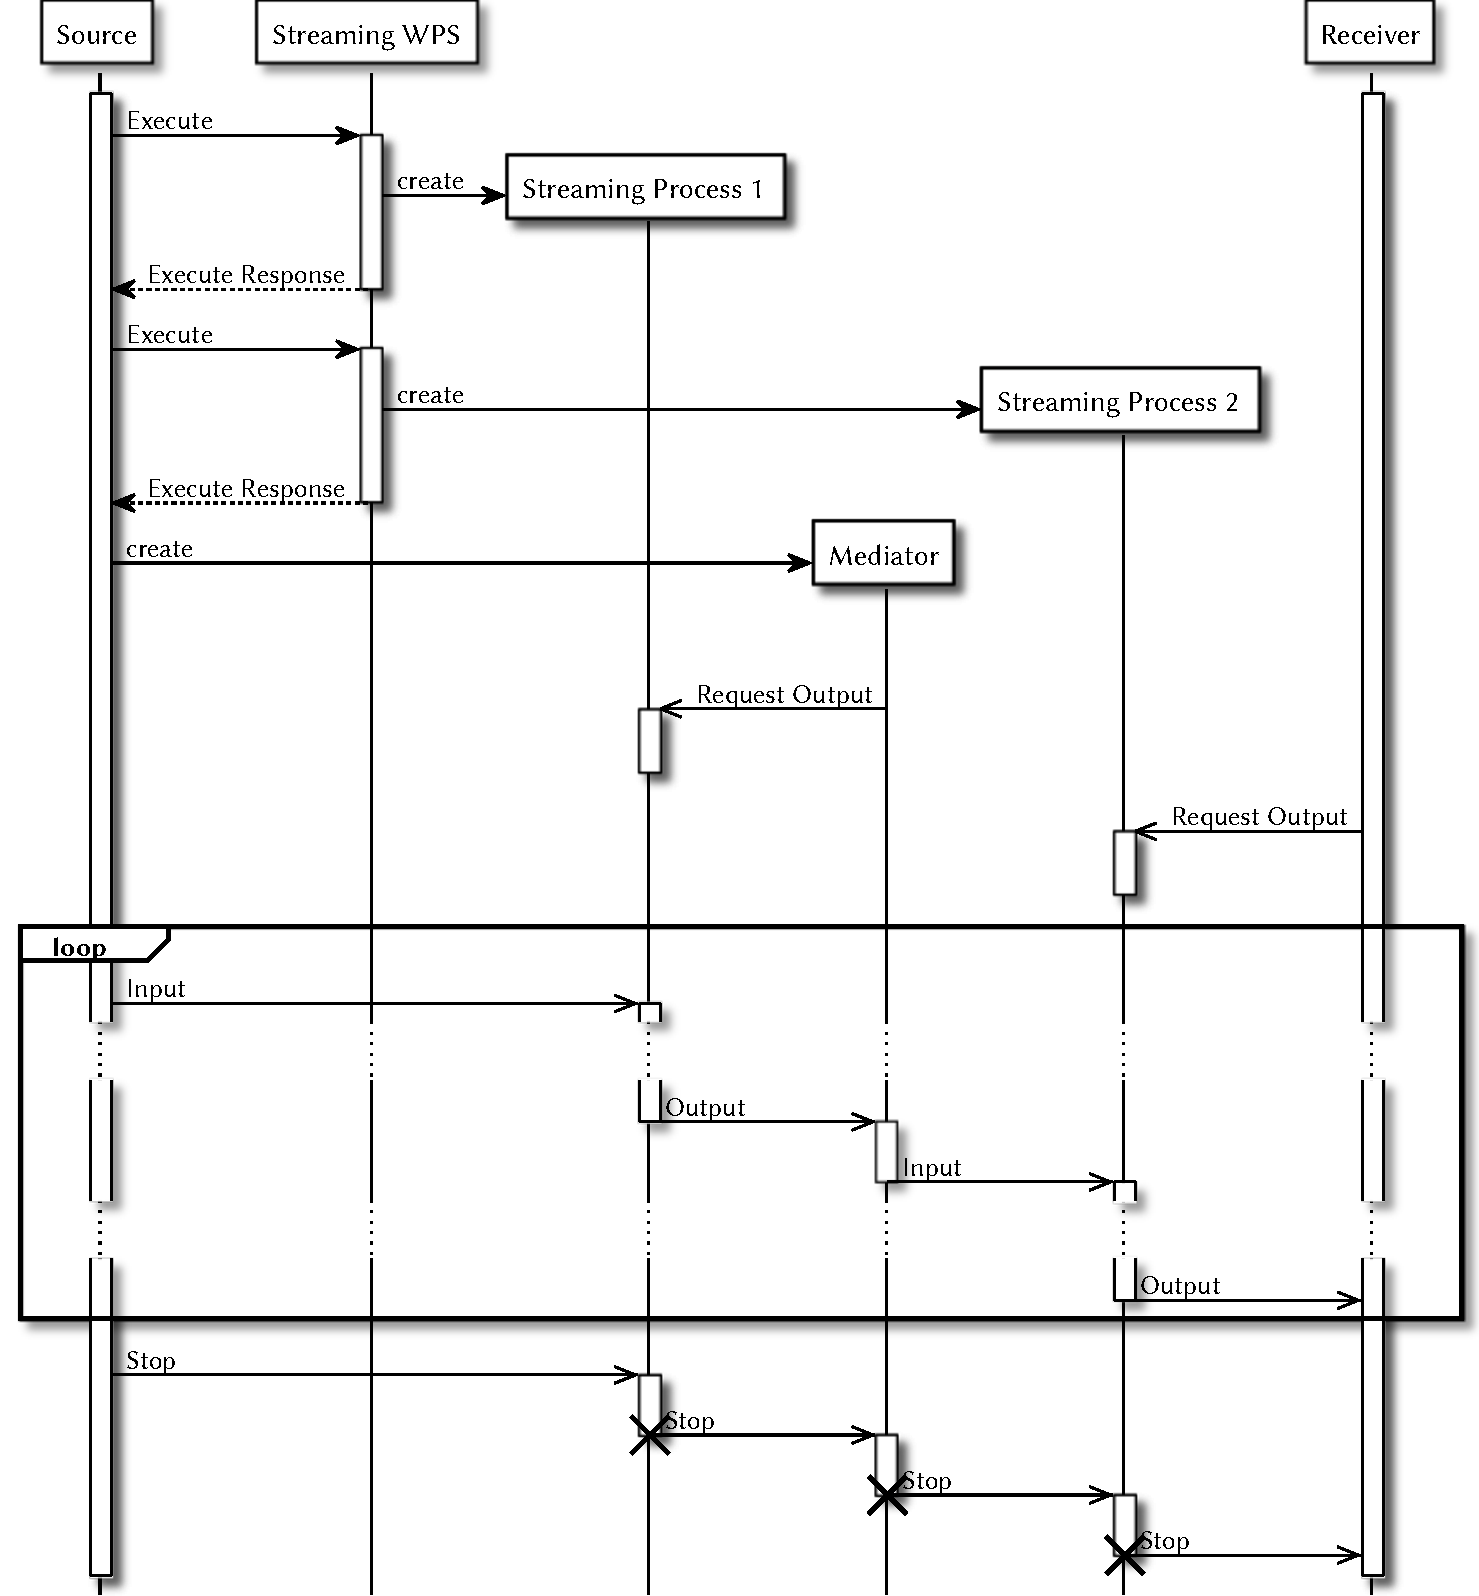
\includegraphics[width = 1\linewidth]{figures/sequence-diagram-chain.pdf}
    \caption{\label{fig:sd:chain}Sequence diagram of chaining two streaming processes using a generic mediator between the processes to translate output to input messages.}
  \end{figure}

  The protocol also enables the chaining of processing steps. This can be realized in two ways: on the one hand, a delegate itself may represent a \ac{WPS} process chain and thus chain every processing step, or, on the other hand, several streaming processes are chained. A simple mediator is translating input messages to output messages (see \cref{fig:sd:chain}). This mediator can be realized using a dedicated streaming enabled algorithm accepting an input/output mapping and the connection parameters of the streaming processes to connect. After requesting the outputs of the source streaming process, it can translate every output message to an input message and forward the stop message. A receiving client will connect to the second streaming process and receives the data process by the chain. By requesting the outputs of the first streaming process, even intermediate results of the chain are accessible.

\section{Messages}
  \label{sec:streaming:messages}
  To fulfill the above defined protocol, several messages have to be exchanged between sender, streaming process and receiver. In order to correlate input and outputs or to show the source of an error, the message format has to have a concept of message references. WebSockets do not have such a concept as it is only a thin layer on top of TCP, which introduces only a handshake and addressing mechanism to be compatible with HTTP and a minimal framing of messages. This framing is merely needed to establish a message-based instead of a stream-based protocol, as the latter would make it hard to differentiate between individual messages \citep{ietf:rfc6455}. To enable referencing of messages, and by this an asynchronous reply mechanism, another layer is needed. As the \ac{WPS} is mostly based on \ac{XML}, the message format should also be \ac{XML}-based. This enables the usage of large parts of the \ac{WPS} schema and allows the reuse of many components written to interact with the \ac{WPS}.

  The widely known SOAP protocol \citep{w3c:soap1} -- which may also be used as an optional binding of the \ac{WPS} \citep{ogc:wps} and thus can be easily adopted -- is an ideal candidate for this. In combination with \ac{WSA} \citep{w3c:wsa} it creates an \ac{XML}-based message framework, which allows asynchronous requests and responses over an arbitrary protocol. Besides introducing a concept of addressing and routing of messages (that will not be used in the Streaming \ac{WPS}), one can assign a globally unique identifier to any message using \ac{WSA}, which can be referenced with arbitrary semantics (e.g. reply).

  The Streaming \ac{WPS} defines seven SOAP messages. These are outlined in the following sections.

  \subsection{Input Message}
    Input messages are used by clients to supply subsequent inputs to a streaming iteration of a streaming process. They loosely resemble a \ac{WPS} Execute request by consisting of any number of inputs and an identifier, that references the streaming process to which the inputs should be supplied. An example can be seen in \cref{lst:streaming:message:input}; possible inputs are discussed in depth in \cref{sec:streaming:input}.
    \lstinputlisting[label={lst:streaming:message:input},
             caption={[Example for a Streaming WPS input message.]Example for a Streaming WPS input message (see \cref{sec:xmlnamespaces} for omitted XML namespaces).},
             language=XML]{listings/streaming-message-input.xml}

  \subsection{Output Messages}
    Output messages are used by the streaming process to transport intermediate results at the end of a streaming iteration or a final result at the end of the streaming process to listening clients. They loosely resemble a \ac{WPS} Execute response by containing an arbitrary number of outputs and the identifier of the process that produced the outputs. Output messages containing intermediate results are replies to their corresponding input message and reference them using \ac{WSA}. If the processing used the output of any other streaming iteration (see \cref{sec:stream:input:reference,sec:stream:dependencies}), the corresponding output messages are also referenced. An example can be seen in \cref{lst:streaming:message:output}.
    \lstinputlisting[label={lst:streaming:message:output},
             caption={[Example for a Streaming WPS output message.]Example for a Streaming WPS output message (see \cref{sec:xmlnamespaces} for omitted XML namespaces).},
             language=XML]{listings/streaming-message-output.xml}

  \subsection{Output Request Message}
    An output request message is used by a client to subscribe to the outputs generated by a streaming process. There is no direct counter part in the \ac{WPS} specification but the concept is similar to the continuous request of the \ac{WPS} response during an asynchronous process execution. As WebSockets offer a full-duplex messaging channel, a continuous polling of outputs is not needed, but the streaming process can push outputs directly to listening clients. To initialize this listening, the client registers to one or more streaming processes using their corresponding identifiers. An example can be seen in \cref{lst:streaming:message:output-request}.
    \lstinputlisting[label={lst:streaming:message:output-request},
             caption={[Example for a Streaming WPS output request message.]Example for a Streaming WPS output request message (see \cref{sec:xmlnamespaces} for omitted XML namespaces).},
             language=XML]{listings/streaming-message-output-request.xml}

  \subsection{Stop Message}
    As streaming processes can run indefinitely long, input supplying clients need to be able to inform the streaming process that there will be no further inputs that become available. To achieve this, a stop message (see \cref{lst:streaming:message:stop}) is sent to the streaming process. The process will propagate the stop message to all listening clients to notify them that there will be no further outputs. Before the stop message is propagated, all streaming iterations that are not yet processed will be finished, but the process will not accept any further inputs. If there are still unresolved dependencies (see \cref{sec:stream:input:reference,sec:stream:dependencies}), the streaming process will fail with an error message.
    \lstinputlisting[label={lst:streaming:message:stop},
             caption={[Example for a Streaming WPS stop message]Example for a Streaming WPS stop message (see \cref{sec:xmlnamespaces} for omitted XML namespaces).},
             language=XML]{listings/streaming-message-stop.xml}

  \subsection{Error Message}
    Errors are transported, as in the \ac{WPS} specification, using \ac{OWS} exception reports \citep{ogc:ows,ogc:wps}. If the delegate of a process fails or a supplied input message can not be processed due to whatever conditions, the error is propagated to listening clients. The error is always sent to the client that sent the message causing the error (if the client is still connected), and in case the error is caused during the execution of a streaming iteration, also to all listening clients that registered through an output request message. In contrast to failures during input validation, e.g. due to constraints imposed by dependencies (see \cref{sec:stream:input:reference,sec:stream:dependencies}), errors raised during the execution of a streaming iteration can not be compensated, but will stop the streaming process. The causing message of a failure may be obtained from the reply relation encoded using \ac{WSA}. An example of an error message can be found in \cref{lst:streaming:message:error}.
    \lstinputlisting[label={lst:streaming:message:error},
             caption={[Example for a Streaming WPS error message.]Example for a Streaming WPS error message (see \cref{sec:xmlnamespaces} for omitted XML namespaces).},
             language=XML]{listings/streaming-message-error.xml}

  \subsection{Describe \& Description Message}
    Describe messages are directly adopted from the \ac{WPS} \emph{DescribeProcess} operation. Due to conditions described in \cref{sec:stream:processdescription}, a client needs to be able to retrieve a description from a running streaming process. The message simply contains the identifier of the process the client wants to have the description from. An example for this process can be seen in \cref{lst:streaming:message:describe}.
    \lstinputlisting[label={lst:streaming:message:describe},
             caption={[Example for a Streaming WPS describe message.]Example for a Streaming WPS describe message (see \cref{sec:xmlnamespaces} for omitted XML namespaces).},
             language=XML]{listings/streaming-message-describe.xml}
    The reply resembles a \emph{DescribeProcess} response and is encoded in a description message referencing the describe message and containing the streaming process description (see \cref{lst:streaming:message:description}).
    \lstinputlisting[label={lst:streaming:message:description},
             caption={[Example for a Streaming WPS description message.]Example for a Streaming WPS description message (see \cref{sec:xmlnamespaces} for omitted XML namespaces).},
             language=XML]{listings/streaming-message-description.xml}

\section{Input Types}
  \label{sec:streaming:input}
  The aforementioned requirements imply three different types of input for a Streaming Process. They differ in the aspect of time (\emph{When are they supplied?}) and scope (\emph{Where are they used?}). Besides that, all of them are based on the very same input types the \ac{WPS} standard defines (see \cref{sec:wps}).
  \subsection{Streaming Inputs}
    \label{sec:streaming:input:streaming}
    The first and most obvious type of input are streaming inputs. They are provided for a single streaming iteration and will only be used in that iteration representing the core of streaming enabled processing (see \cref{lst:streaming:input:streaming}).

    \lstinputlisting[label={lst:streaming:input:streaming},
             caption={[Example for a Streaming WPS streaming inputs.]Example for a Streaming WPS streaming inputs (see \cref{sec:xmlnamespaces} for omitted XML namespaces).},
             language=XML]{listings/streaming-input-streaming.xml}

    A conventional algorithm to compute the histogram of a raster (e.g. a satellite image) needs the complete raster as a single complex input for processing. A streaming enabled variant would split the raster in several smaller tiles and supply each of them in a single input message to the streaming process. The algorithm can process each tile on its own and update the global histogram. Besides that the process does not have to store the complete raster, it is also able to output intermediate histograms to the client.

  \subsection{Static Inputs}
    \label{sec:stream:input:static}
    Algorithms operating on a streaming input often need inputs that are common to every iteration. It would be redundant and inefficient to transfer inputs like configuration parameters in every input message for every streaming iteration. For this, the concept of static inputs needs to be introduced. Static inputs are parameters that are supplied when a streaming process is created and apply to every streaming iteration (see \cref{lst:streaming:input:static}). While the streaming process handles a streaming iteration, the static inputs are merged with the inputs of the causing input message and transparently supplied to the process's delegate. This way, a conventional process can be easily converted into a streaming enabled process. Additionally, static inputs can be handled separately to configure a streaming process's delegate when it is created.

    \lstinputlisting[label={lst:streaming:input:static},
             caption={[Example for a Streaming WPS static inputs.]Example for a Streaming WPS static inputs (see \cref{sec:xmlnamespaces} for omitted XML namespaces).},
             language=XML]{listings/streaming-input-static.xml}

    For example, a traditional process implementation of the Douglas-Peucker algorithm \citep{douglas1973algorithms} would require a feature collection and a $\epsilon$ value as inputs. In a streaming environment, one would model the $\epsilon$ input as a static input supplied at process creation and stream the feature collection as single features in streaming inputs. Other examples are a coordinate transformation process that accepts a feature collection and a target \ac{CRS}, or a buffer algorithm that accepts a feature collection and a buffer size. Buffer size and \ac{CRS} would be supplied as static inputs, whereas the feature collection would be split into several streaming inputs and would be supplied in independent streaming iterations.

  \subsection{Reference Inputs}
    \label{sec:stream:input:reference}
    While streaming offers no real benefit to algorithms that require global knowledge of the data set, there are often cases where algorithms only require knowledge about few other chunks of the data set or even only about the result of their processing. To model these dependencies between streaming iterations, reference inputs can be used (see \cref{lst:streaming:input:reference}). These reference the output of another -- previous or upcoming -- iteration as an input parameter. Reference inputs break out of the conventional non-random access paradigm of streaming and allow a semi-random access processing of a data set. Inputs are described by referencing the corresponding output identifier and the input message that has or will produce the output data. The order of incoming input messages is irrelevant to the use of reference inputs, as input messages referencing not yet available outputs will be delayed until they can be processed (see \cref{sec:stream:dependencies}).

    \lstinputlisting[label={lst:streaming:input:reference},
             caption={[Example for a Streaming WPS reference input.]Example for a Streaming WPS reference input (see \cref{sec:xmlnamespaces} for omitted XML namespaces).},
             language=XML]{listings/streaming-input-reference.xml}

    A conventional algorithm to analyze a river system, in which each processing of a river depends on the processing results of the rivers flowing into it, the complete river system data set would be supplied as a single input parameter. In a streaming enabled process, each river would be supplied as a streaming input. The output of the rivers that a river depends on would be supplied as additional reference inputs.

  \subsection{Polling inputs}
    \label{sec:stream:input:polling}
    The last category of possible input types for a streaming \ac{WPS} are polling inputs. These inputs are continuously polled from an external resource and a new streaming iteration would be started, when new inputs become available. Polling inputs would be supplied at process creation time and would contain a reference to an external resource, which is requested continuously. In order to not miss inputs when they become available, a playlist file as described in previous approaches \citep{foerster2012live} would be needed. The implementation of polling inputs as part of this streaming \ac{WPS} specification would present the very same issues that were criticized in previous approaches:
    \begin{itemize}
      \item How can polling frequencies used to retrieve the playlist be defined?
      \item How can multiple polling inputs be declared?
      \item How would they be combined by the streaming \ac{WPS}?
    \end{itemize}
    For this reason, the Streaming \ac{WPS} will not implement polling inputs. These input types are by far better handled on client side, as the client typically knows the rate data becomes available. By this the client can choose an appropriate polling frequency and also is able to coordinate multiple polling inputs by having a deeper understanding of their affiliation. Polling inputs could be implemented as shown in \cref{fig:sd:polling}: the client polls a data provider (e.g. a \acrocitep{SOS}{ogc:sos}) to check if new data is available and convert this data into a streaming input for the Streaming \ac{WPS}.

    \begin{figure}[!htb]
      \centering
      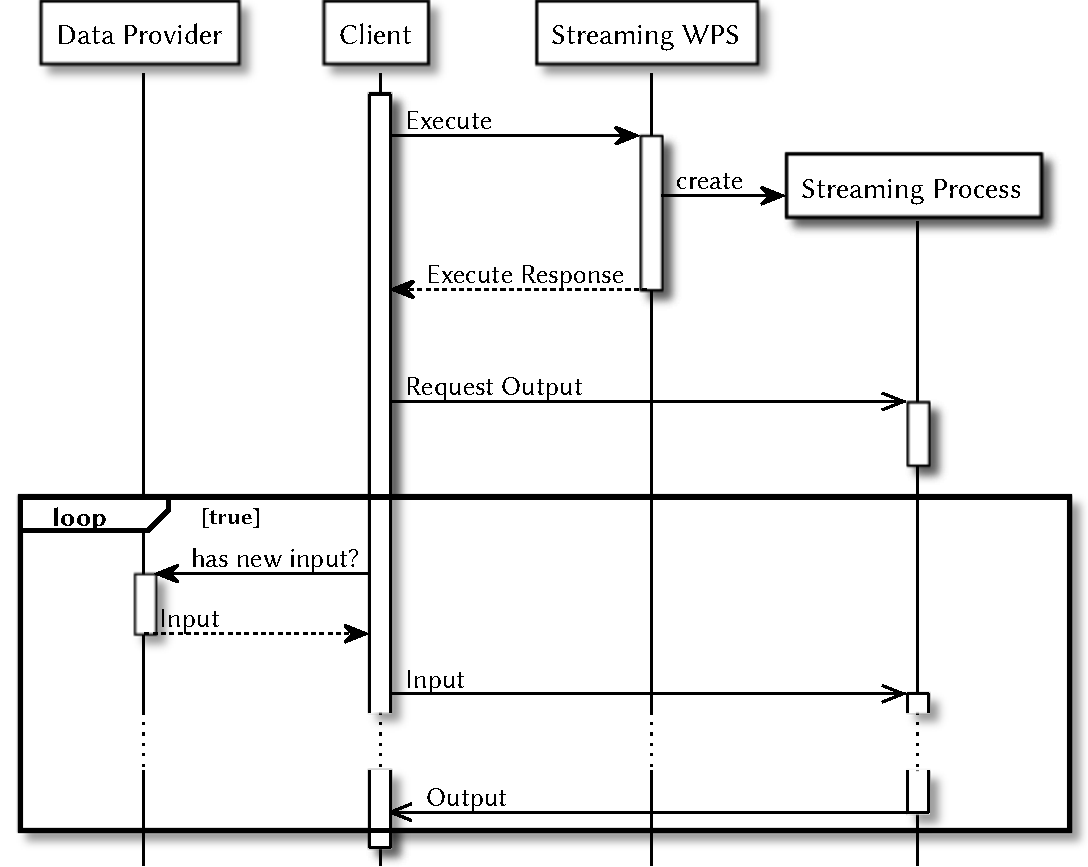
\includegraphics[width = 0.73521126760563382\linewidth]{figures/sequence-diagram-polling.pdf}
      \caption{\label{fig:sd:polling}Sequence diagram of how to implement polling inputs for a streaming enabled WPS algorithm.}
    \end{figure}

\section{Dependencies}
  \label{sec:stream:dependencies}
  The definition of reference inputs in \cref{sec:stream:input:reference} implies a mechanism to resolve dependencies and to order the execution of streaming iterations. These are considered as tasks and can declare dependencies to other streaming iterations either by mapping an input to the output of another streaming iteration or by declaring an explicit dependency on another streaming iteration.

  Dependencies can be best modeled using a \ac{DAG}. A \ac{DAG} is a structure $D=(V, E)$ consisting of a set of vertices (or nodes) $V$ and edges (or arcs) $E$ where every edge $e\in E$ is a ordered tuple $v_1 \rightarrow v_2$ with $v_1, v_2 \in V$. The distinct vertices $v_1,\dots,v_n\in V$ are called a path if for all successive vertices $v_i, v_{i+1}$ exists an edge $v_i \rightarrow v_{i+1} \in E$. A directed graph is called acyclic if there exists no path in $G$ with $v_1 = v_n$ \citep{jungnickel2012graphs}. A subgraph of a graph is the graph $G' = (V', E')$ with $V'\subseteq V$ and $E' = \{v_1 \rightarrow v_2 \in E | v_1, v_2\in V'\}$. Two subgraphs $G_1 = (V_1, E_1), G_2 = (V_2, E_2)$ are independent if $V_1 \cap V_2 = \emptyset$ and there exists no edge $v_1\rightarrow v_2\in E$ with $v_1\in V_1 \wedge v_2\in V_2$ or $v_2\in V_1 \wedge v_1\in V_2$.

  In a dependency graph, vertices represent a task, package or other entity that has dependencies, and edges represent these dependencies ($v_1$ depends on $v_2$). Dependency graphs have to be acyclic as a cycle would introduce a cyclic dependency that can not be resolved.

  \begin{figure}[!htb]
    \centering
    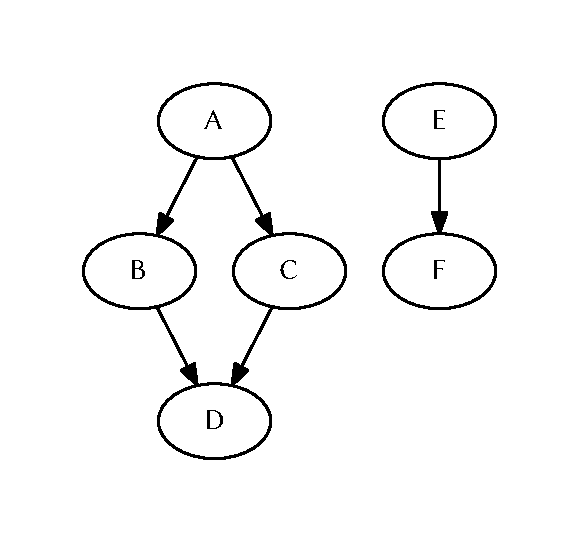
\includegraphics[width = 0.44694533762057875\linewidth]{figures/unordered-graph.pdf}
    \caption{\label{fig:graph:unordered}Example for a dependency graph consisting of two independent subgraphs. Arrows denoting a dependency between the nodes.}
  \end{figure}

  A system containing the tasks $A, B, C, D, E, F$ and the dependencies $A\rightarrow B, A\rightarrow C, B\rightarrow D, C\rightarrow D$ and $E\rightarrow F$ will result in a \ac{DAG} consisting of two independent subgraphs (see \cref{fig:graph:unordered}).

  The execution order of a dependency graph can be derived from the topological ordering of the graph: a ``topological ordering, $ord_D$, of a directed acyclic graph $D = (V, E)$ maps each vertex to a priority value such that $ord_{D}(x) < ord_{D}(y)$ holds for all edges $x \rightarrow y \in E$'' \citep{pearce2007dynamic}. A possible execution order is the list of all vertices sorted by descending $ord_D$. The topological order of a \ac{DAG} can be computed using e.g. \ac{BFS} in linear time \citep{cormen2001introduction}. In most cases, the topological ordering is not unique; \cref{fig:graph:ordered} shows one possible execution order for the before mentioned graph.

  \begin{figure}[!htb]
    \centering
    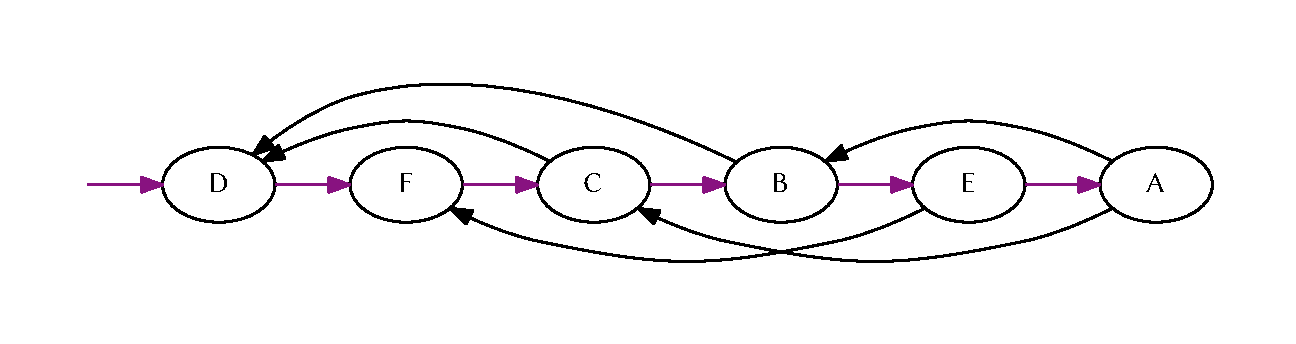
\includegraphics[width = 1\linewidth]{figures/ordered-graph.pdf}
    \caption{\label{fig:graph:ordered}Possible execution/topological order of the dependency graph in \cref{fig:graph:unordered}. Black arrows represent dependence to another vertex, colored arrows the execution order.}
  \end{figure}

  In contrast to conventional dependency systems like package managers, the Streaming \ac{WPS} can not operate on a static graph of dependencies but on a graph to which vertices and edges are added constantly. Conventional topological sorting algorithms have to recompute the ordering for every insertion from scratch, which will have a big performance impact for the scenario of a great number of small streaming iterations. There exist a few dynamic topological sort algorithms that will maintain the topological order across edge and node insertions, and will only recompute the ordering if necessary.

  Most dependency graphs generated using the Streaming \ac{WPS} will probably consist of multiple independent subgraphs, no dependencies at all would be the most extreme example, or quite sparse graphs. For this, the algorithm described by \citet{pearce2007dynamic} seems to be appropriate. Even though it is theoretically inferior to other algorithms for dynamic topological sorting \citep[e.g. ][]{alpern1990incremental,marchetti1996maintaining}, in practice it performs better especially on sparse graphs and on dense graphs only a constant factor slower than other algorithms \citep{pearce2007dynamic}.

  Dependencies are of particular importance in case of execution failures. If the computation of a streaming iteration fails for whatever reason, all iterations that directly or indirectly depend on this iteration can not complete. As this also holds true for iterations that are supplied at a later time in the streaming process, the process can not proceed ignoring the error. Due to this, every error that occurs during the execution of a streaming iteration results in the termination of the streaming process.
  Dependencies also have a special meaning at the end of a streaming process, when a stop message is sent to notify the streaming process to accept no further inputs and finish pending streaming iterations. At this point, all dependencies need to be able to be satisfied, which implies that all referenced input messages have been sent to the streaming process. In case a referenced input message is missing, the service is not able to complete gracefully and will fail. As references to future streaming iterations are allowed, prior to this point it is not possible for the Streaming \ac{WPS} to determine if a reference may not be fulfilled. Because the service is not able to fail fast for incorrect references, clients using dependencies between streaming iterations have to pay careful attention to references.

  It should also be noted, that the smallest unit that can be referenced in a streaming process is the output of a streaming iteration. Format specific references, e.g. to a particular feature inside a feature collection, are not possible using this protocol. Because of that, streaming process implementations need to be designed to not require smaller components or have to deploy an own referencing strategy (e.g. by supplying an additional input to identify the feature of the referenced collection). But, as this results in superfluous transfer of data, such solutions should be avoided. One may point out, that there is no way to reference input parameters of other streaming iterations, but this use case should be already covered by the \ac{WPS}'s own input reference parameters (see \cref{sec:streaming:input}).

\section{Process Description} % TODO proof read
  \label{sec:stream:processdescription}
  The conventional process description mechanism of the \ac{WPS} is not sufficient to describe streaming processes.

  It consists of a \emph{DescribeProcess} request issued to the \ac{WPS} and the retrieval of one or more process descriptions of the specified process. These descriptions contain detailed descriptions of input and output parameters of the process and information about the supported formats, units of measurement or coordinate reference systems of each parameter. They also include details about allowed values, default value and multiplicity of input parameters \citep{ogc:wps}.

  Because the Streaming \ac{WPS} uses the \ac{WPS} interface only to start a Streaming Process and the \ac{WPS} interface does not provide any extension points for process descriptions, the \emph{DescribeProcess} operation can only be used to describe the starting process, but not the input or output parameters of a streaming process.

  In case of generic processes, e.g. processes that delegate to other \ac{WPS} processes, information about input and output parameters is not even available prior to the execution of the streaming process. Furthermore input parameter cardinalities may change due to the use of static inputs. By this a valid input parameter for a delegate process may not be used in subsequent inputs because the maximal occurrence of the parameter is already exhausted using static input parameters. By this a process description for a streaming process will always be instance specific and can not be generated by the associated \ac{WPS} process.

  With knowledge of the delegate process a client may have enough information to facilitate the streaming process but for other streaming process there is no way for a generic client to know the input parameters of the process.

  To compensate this shortcoming a method is needed to describe a Streaming Process instance at runtime.

\section{Implementation}
  The Streaming WPS was prototypically, but feature complete implemented as a module for the \ftn WPS implementation. Besides offering a framework to develop all kinds of streaming enabled processes, it features a generic streaming process implementation that is able to convert every suitable algorithm (e.g. Douglas–Peucker) into a streaming enabled variant. The generic streaming process accepts the description of another WPS process and the URL of its endpoint as input parameters, and uses this remote process as an delegate for every streaming iteration. Additionally, it accepts a collection of static input parameters that are merged with the input parameters of a streaming iteration and are then transparently sent to the delegate process in every streaming iteration. Processes developed using the framework are able to maintain an internal state that can be mutated during execution, e.g. to create the sum of all streaming iterations, which is outputted as a final result. Due to the fact that the WPS standard defines a stateless protocol, whereas the protocol defined by the Streaming WPS encourages the use of an internal state, the possibilities of the generic streaming process are limited in this regard. Internal state can only be conveyed using the dependency mechanisms provided by the Streaming WPS, i.e. transporting state in input and output parameters.

  % !TEX root = ../thesis.tex

\begin{figure}
  \def\fibfigsize{1\linewidth}
  \centering
  \begin{subfigure}{\fibfigsize}
    \caption{Starting of the streaming process using a WPS \emph{Execute} request, requesting of the streaming process's description and supplying of three input messages, of which only $fib(0) = 0$ can be processed immediately.}
    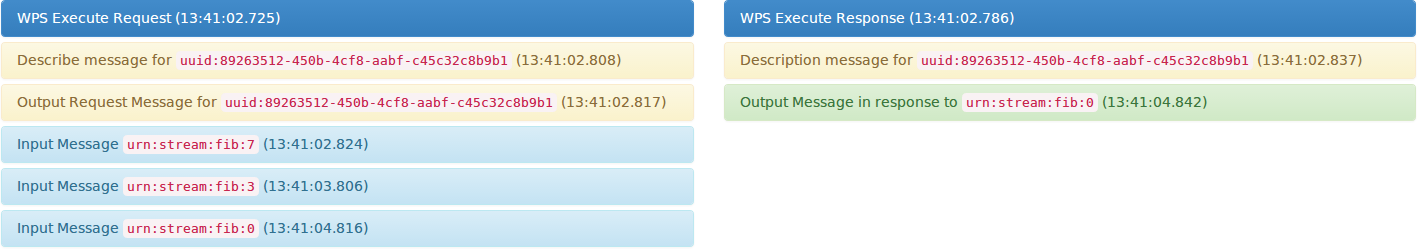
\includegraphics[width = \linewidth]{figures/fibonacci-1.png}
  \end{subfigure}
  \begin{subfigure}{\fibfigsize}
    \caption{$fib(1) = 1$ is supplied in an input message, and so the previously supplied request for $fib(2)$ and $fib(3)$ can be calculated. $fib(7)$ is still missing prerequisites.}
    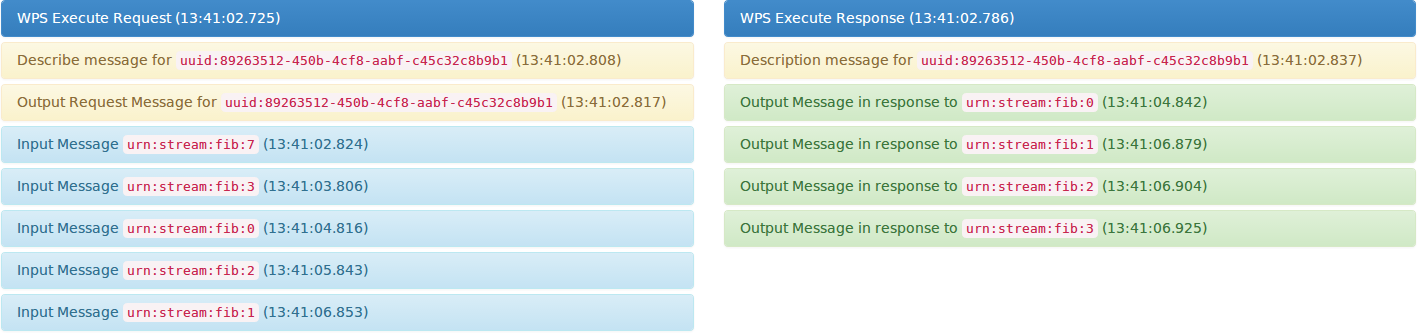
\includegraphics[width = \linewidth]{figures/fibonacci-2.png}
  \end{subfigure}
  \begin{subfigure}{\fibfigsize}
    \caption{As the dependencies of $fib(4)$ and $fib(5)$ are fulfilled, they can directly be calculated. $fib(7)$ is still missing the result of $fib(6)$.}
    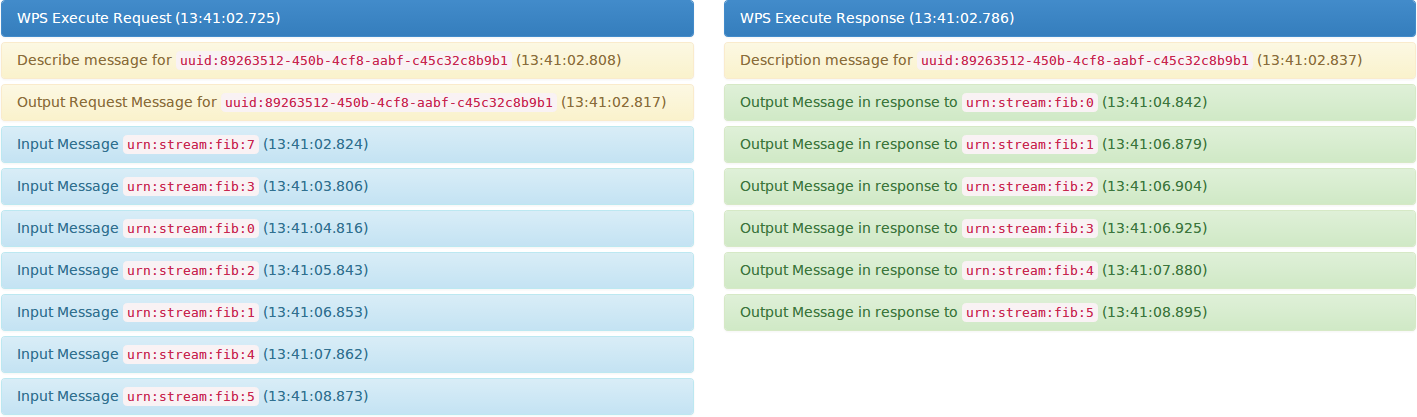
\includegraphics[width = \linewidth]{figures/fibonacci-3.png}
  \end{subfigure}
  \begin{subfigure}{\fibfigsize}
    \caption{At the time the request for $fib(6)$ arrives, all preconditions are met and $fib(6)$ and the final $fib(7)$ can be calculated. Once the result has arrived, the client stops the streaming process.}
    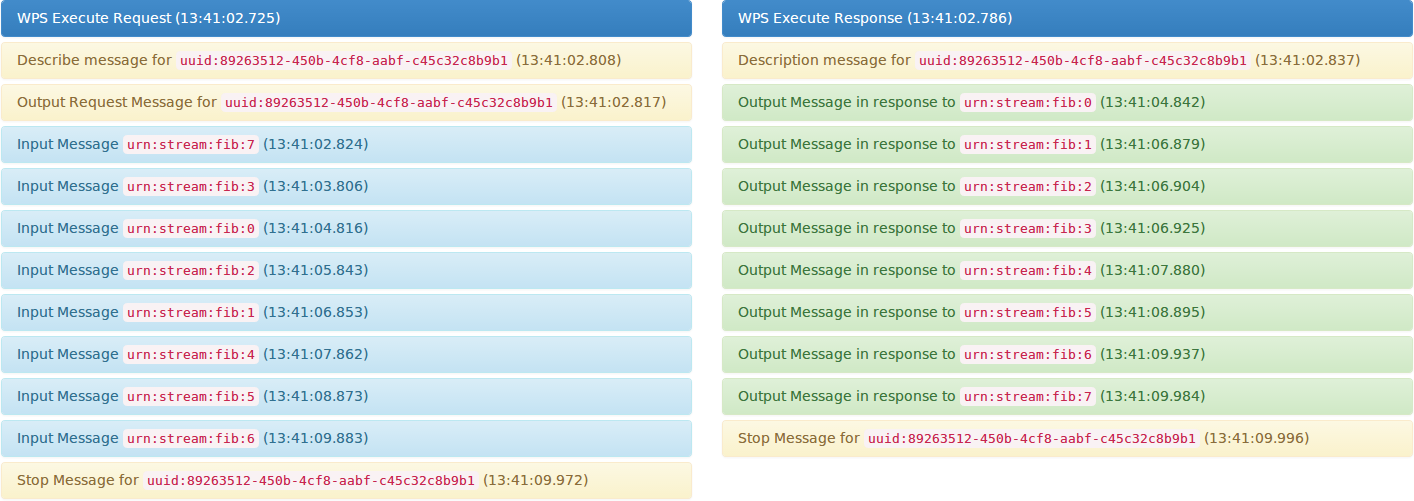
\includegraphics[width = \linewidth]{figures/fibonacci-4.png}
  \end{subfigure}
  \caption{\label{fig:client}Calculation of the seventh Fibonacci number using the Streaming WPS, its accompanying JavaScript API and a simple addition WPS process as the streaming process's delegate.}
\end{figure}

  An example for this can be visualized using the JavaScript-based client library that was developed. The \acs{API} abstracts message encoding and WebSocket interaction, allows to start and stop streaming processes, to supply input messages, to request the process's description as well as to retrieve outputs. A basic demonstration of the Streaming WPS's capabilities can be seen in \cref{fig:client}, in which the seventh Fibonacci number is calculated using a streaming process. Fibonacci numbers are the values of the integer sequence $0, 1, 1, 2, 3, 5, 8, 13, \dots$ defined inductively by the function $fib(n) = fib(n-1) + fib(n-2)$ with $fib(0) = 0$ and $fib(1) = 1$. $fib(n)$ is thereby called the \emph{n-th Fibonacci number} \citep{fibonacci}. Through their recursive definition, Fibonacci number calculation can be used to showcase the advanced dependency resolution capabilities of the Streaming WPS. The generic streaming process is started with a reference to another WPS process, which sole functionality is to add two integers and to return the result. Each Fibonacci number is then defined in its own streaming iteration by supplying an input message to the streaming process. To break down the principle of calculating Fibonacci numbers to the addition of two numbers, $fib(0)$ is defined as the addition of $0$ and $0$ and $fib(1)$ as the addition of $0$ and $1$. All following Fibonacci numbers are defined as the addition of the results of the two previous streaming iterations. By sending the input messages in a random order, the streaming process has to postpone calculation of a streaming iteration until the input messages of the two referenced streaming iterations have arrived and their results are available. This can be seen from the intermediate results containing all Fibonacci numbers previous to the one requested that arrive in order.

\section{Streaming \la WPS}
  The implementation of a streaming variant of the \la process presented in \cref{sec:matlab:la} has to be divided in two different use cases. Processing of large data sets of several lakes can be easily accomplished using the generic streaming process implementation presented in the previous section. Configuration parameters for down-sampling rates, error correction and plotting configuration can be supplied using static input parameters, whereas the streaming input messages contain bathymetry, wind and water measurements and optionally salinity information. In this case, the greater data set of time series for multiple lakes is broken into smaller chunks spatially, whereas the temporal dimension is not modified.

  By splitting a data set temporally, the analysis of very long time series or near real time buoys data is possible. In theory, streaming chunks can be reduced to a single point in time by deactivating the down sampling code of the \la. This would allow to offer characteristics as single values instead of \ac{CSV} files. Because the \la can not maintain state across streaming iterations but has to operate on a single point in time, error checking, outlier detection and temporal averaging would not be possible using the \la as a delegate to the generic streaming process. By this, outputs like Lake or Wedderburn Number are more prone to error or may not be meaningful, e.g. mode-1 vertical seiche period. Development of a stateful streaming process that overcomes this issues would, however, neglect the efforts and possibilities already done in the \la.

  An easier solution to enable near real time or live analysis is to find an appropriate time frame adapted to the sampling rate of sensors deployed in a lake, which is large enough to allow temporal averaging and error checking but is small enough to produce continuous outputs. This approach could be realized using the generic streaming algorithm implementation: the process is initialized using a reference to the \la process, and bathymetry, configuration parameters and plotting parameters are supplied as static inputs. Water temperature, wind speed and optionally level and salinity measurements are supplied in each streaming iteration. The supplied time frame should ideally be chosen such that after down sampling, smoothing and error correction only a single point in time is outputted.

  Future extensions of the \la, e.g. calculations of parameters that require the previous results, or analysis of chains of lakes in which lakes depend on each other, could also be easily realized. By implementing previous results or the results of a previous lake in the chain as additional inputs to the \la, these dependencies can be easily resolved by the streaming process.